\section{Experiments}
\label{sec:experiments}

The experiments address three mechanism questions. First, under controlled nonlinear residuals,
does NTD-PL behave as intended: remaining close to Tucker in the linear regime while gaining
when the residual is link-like and the active polynomial degree is expressive enough? Second,
on real hyperspectral tensors, does the polynomial link provide a compact fixed-backbone
enhancement that improves both representation and held-out completion, rather than merely
spending more parameters? Third, can a frozen-backbone Link Refresh diagnostic identify, before
full NTD-PL training, which tensor units contain residual structure that a scalar link can exploit?
Unless stated otherwise, real tensors are globally max-normalized and used without spatial
downsampling or cropping. We report $RMSE$ and $SAM$ for reconstruction, and $RMSE^*$ and
$SAM^*$ only on held-out entries for completion. NTD-PL is compared mainly against same-rank
Tucker, except in the rank-lift ablation.

\subsection{Controlled Nonlinear Residuals}
\label{subsec:controlled-experiments}

These synthetic experiments are mechanism checks rather than generic
benchmarks. We generate measured tensors as
\[
Y_\alpha=\sqrt{1-\alpha}S^\star+\sqrt{\alpha}\widetilde{R}^\star,
\]
where \(S^\star\) is a low-rank Tucker tensor and \(\widetilde{R}^\star\) is
the normalized component of a scalar nonlinear response orthogonal to
\(S^\star\). Thus \(\alpha\) controls nonlinear residual energy, not just the
raw amplitude of a nonlinearity. Figure~\ref{fig:controlled-alpha-grid} shows
the expected transition: NTD-PL is Tucker-like when the residual is nearly
linear and separates as nonlinear residual energy increases. Tucker can lag
behind CP, but NTD-PL then pulls ahead systematically.
Figure~\ref{fig:controlled-pmax-strip} shows the complementary degree effect:
gains emerge when the active polynomial degree can match or approximate the
response complexity. Degree continuation and coefficient-contribution details
are deferred to Appendix~\ref{app:controlled-synthetic}, where Table~\ref{tab:linear-consistency-controlled} shows the linear consistency negative control.

\begin{figure}[!htbp]
  \centering
  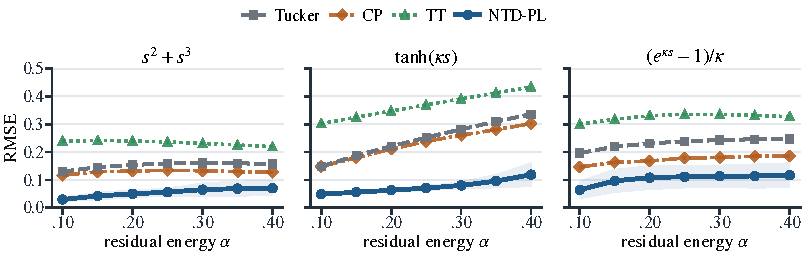
\includegraphics[width=0.98\linewidth]{figures/controlled_nonlinear_alpha_grid.pdf}
  \caption{Controlled nonlinear residual sweep. NTD-PL stays Tucker-like near
  the linear regime and separates as \(\alpha\), the nonlinear residual energy,
  increases. Lower RMSE is better.}
  \label{fig:controlled-alpha-grid}
\end{figure}

\begin{figure}[!htbp]
  \centering
  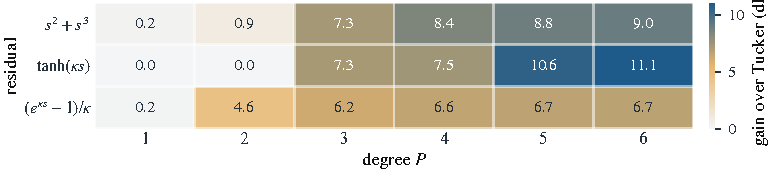
\includegraphics[width=0.98\linewidth]{figures/controlled_nonlinear_pmax_heatmap.pdf}
  \caption{Degree-dependent gains at \(\alpha=0.25\). Cell values are Tucker
  minus NTD-PL RMSE; gains appear when the active degree is sufficient for the
  response complexity.}
  \label{fig:controlled-pmax-strip}
\end{figure}

Taken together, these controlled experiments answer the first question. NTD-PL does not obtain
gains simply by adding a polynomial link: it stays close to Tucker when the source is linear or
nearly linear, and its advantage appears when the residual is both nonlinear and expressible by
the active degrees. The synthetic results therefore isolate the intended mechanism before moving
to real tensors.

\FloatBarrier

\subsection{Tucker Enhancement on Real Hyperspectral Tensors}
\label{subsec:lowrank-completion}

This section tests the same fixed-rank enhancement on real hyperspectral
tensors, in both full reconstruction and held-out completion. We use CAVE
\citep{cave_multispectral_database,yasuma2010gapc}, whose multiple real scenes
provide a compact spectral-spatial mechanism check.

\paragraph{Representation enhancement.}
Full reconstruction checks representation capacity rather than generalization.
Figure~\ref{fig:cave-reconstruction-capacity} shows that, at matched Tucker
backbone rank and similar parameter budget, NTD-PL reduces RMSE and SAM. The
gap shrinks as Tucker rank grows, while Table~\ref{tab:rank-lift-tucker} shows
that Tucker needs substantially more rank and parameters to match NTD-PL RMSE.
NTD-PL also usually keeps a clearer SAM advantage.

\begin{figure}[!htbp]
  \centering
  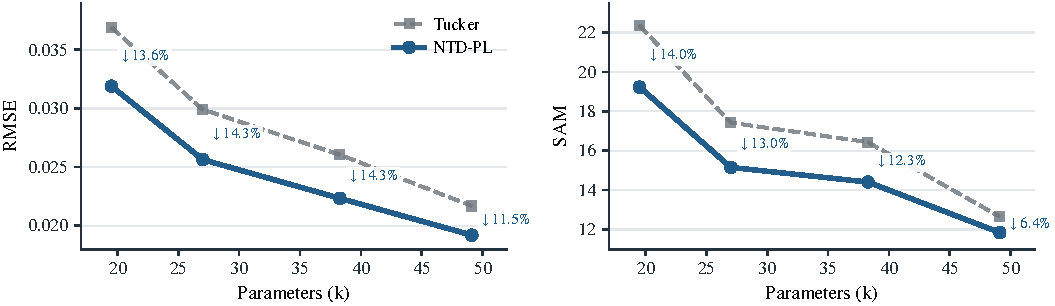
\includegraphics[width=0.98\linewidth]{figures/cave_reconstruction_capacity.pdf}
  \caption{CAVE full reconstruction. At matched backbone rank, NTD-PL reduces
  RMSE and SAM; annotations show paired gains over Tucker. The gap narrows with
  Tucker rank, consistent with fixed-rank enhancement. Points average 15
  scenes.}
  \label{fig:cave-reconstruction-capacity}
\end{figure}

\begin{table}[!htbp]
  \centering
  \caption{Rank-lifted Tucker comparison on CAVE reconstruction. For each
  NTD-PL backbone rank, we report the first higher-rank Tucker model matching
  NTD-PL RMSE and its extra parameters.}
  \label{tab:rank-lift-tucker}
  \scriptsize
  \resizebox{\linewidth}{!}{\begin{tabular}{@{}l r cc l r cc r@{}}
\toprule
\multicolumn{4}{c}{NTD-PL reference} &
\multicolumn{4}{c}{First fixed-channel Tucker matching RMSE} & Extra \\
\cmidrule(lr){1-4}\cmidrule(lr){5-8}
Rank & Params & RMSE$\downarrow$ & SAM$\downarrow$ &
Rank & Params & RMSE$\downarrow$ & SAM$\downarrow$ & \\
\midrule
\((18,18,3)\) & 20k & 0.0319 & \textbf{19.23} & \((28,28,3)\) & 31k & \textbf{0.0316} & 21.41 & \(+59.5\%\) \\
\((24,24,4)\) & 27k & 0.0256 & \textbf{15.15} & \((35,35,4)\) & 41k & \textbf{0.0254} & 16.26 & \(+51.3\%\) \\
\((33,33,4)\) & 38k & 0.0223 & \textbf{14.41} & \((49,49,4)\) & 60k & \textbf{0.0222} & 15.28 & \(+56.5\%\) \\
\bottomrule
\end{tabular}
}
\end{table}

\paragraph{Held-out enhancement.}
Held-out completion tests transfer to unseen entries. Table~
\ref{tab:lowrank-completion-main} reports random-mask CAVE completion, with
metrics computed only on missing entries. At the same rank budget, NTD-PL gives
consistent RMSE$^\ast$ gains and usually improves SAM$^\ast$; paired sign and
Wilcoxon tests in Appendix~\ref{app:single-rank-completion} show the same
scene-level pattern.

\begin{table}[!htbp]
  \centering
  \caption{Held-out CAVE completion at rank \((33,33,4)\) under random masks.
  Metrics use missing entries only; gains are paired improvements over
  matched-rank Tucker.}
  \label{tab:lowrank-completion-main}
  \scriptsize
  \resizebox{\linewidth}{!}{\begin{tabular}{@{}c c c c c c c@{}}
\toprule
\multirow{2}{*}{\(\rho\)} &
\multicolumn{3}{c}{RMSE*$\downarrow$} &
\multicolumn{3}{c}{SAM*$\downarrow$} \\
\cmidrule(lr){2-4}\cmidrule(l){5-7}
& Tucker & NTD-PL & Gain
& Tucker & NTD-PL & Gain \\
\midrule
0.1 & \(0.0263{\pm}0.0179\) & \(\mathbf{0.0229{\pm}0.0158}\) & 12.9\%
& \(11.82{\pm}5.33\) & \(\mathbf{8.36{\pm}3.38}\) & 29.3\% \\
0.3 & \(0.0263{\pm}0.0179\) & \(\mathbf{0.0230{\pm}0.0158}\) & 12.5\%
& \(14.75{\pm}6.33\) & \(\mathbf{12.47{\pm}5.06}\) & 15.5\% \\
0.5 & \(0.0264{\pm}0.0179\) & \(\mathbf{0.0230{\pm}0.0158}\) & 12.9\%
& \(15.56{\pm}6.85\) & \(\mathbf{13.48{\pm}5.75}\) & 13.4\% \\
0.7 & \(0.0266{\pm}0.0180\) & \(\mathbf{0.0219{\pm}0.0128}\) & 17.7\%
& \(16.02{\pm}7.21\) & \(\mathbf{13.79{\pm}5.43}\) & 13.9\% \\
\bottomrule
\end{tabular}
}
\end{table}

These CAVE results answer the second question. The polynomial link improves matched-rank
Tucker not only as a representation-capacity check, but also on held-out entries under random
missingness. The rank-lift comparison further shows that the gain is not merely a parameter-count
effect: at the same Tucker backbone rank, the tied link supplies a compact nonlinear enhancement
that higher-rank Tucker can only match with substantially more ordinary multilinear capacity.

\FloatBarrier

\subsection{Diagnosing Nonlinear Low-Rank Structure Across Data}
\label{subsec:external-hsi-validity}

NTD-PL is meant to be diagnosable rather than uniformly beneficial: it should
help when matched-rank Tucker leaves residual structure that a scalar link can
reduce. We use \(D_{\mathrm{link}}\) as a cheap frozen-backbone probe: fit
Tucker, apply one Link Refresh step from Section~\ref{sec:optimization}, and
record how much Tucker residual energy this one-step link removes on the
evaluation entries. Appendix~\ref{app:posthoc-calibration-baselines} gives the
exact formula.

For CAVE completion, Table~\ref{tab:cave-link-yield-summary} groups scenes by
\(D_{\mathrm{link}}\) tercile. Higher scores correspond to larger held-out
gains across missing rates, with Spearman correlations around 0.829--0.889;
Appendix Figure~\ref{fig:cave-link-yield-scatter-appendix} gives scene-level
scatters.

\begin{table}[!htbp]
  \centering
  \caption{CAVE completion diagnostic. Scenes are grouped by
  \(D_{\mathrm{link}}\) tercile; entries are mean NTD-PL RMSE$^\ast$ gains over
  matched-rank Tucker.}
  \label{tab:cave-link-yield-summary}
  \small
  \begin{tabular}{@{}c c c c c c@{}}
\toprule
$\rho$ & Spearman $\rho_s$ & Low-score gain & Mid-score gain & High-score gain & Scenes\\
\midrule
0.3 & 0.736 & 7.53\% & 10.67\% & 18.40\% & 15\\
0.5 & 0.671 & 8.18\% & 10.70\% & 18.38\% & 15\\
\bottomrule
\end{tabular}

\end{table}

We apply the same protocol beyond HSI. Figure~
\ref{fig:nonhsi-link-scatter} plots \(D_{\mathrm{link}}\) against RMSE
gain. Across all three families, larger \(D_{\mathrm{link}}\) consistently
identifies units with larger NTD-PL gains; object-view tensors show the
strongest separation, action video follows the same trend, and natural images
retain a positive but lower-yield regime. Appendix Table~\ref{tab:nonhsi-link-diagnostic-stats} gives the numeric statistics behind Figure~\ref{fig:nonhsi-link-scatter}.

\begin{figure}[!htbp]
  \centering
  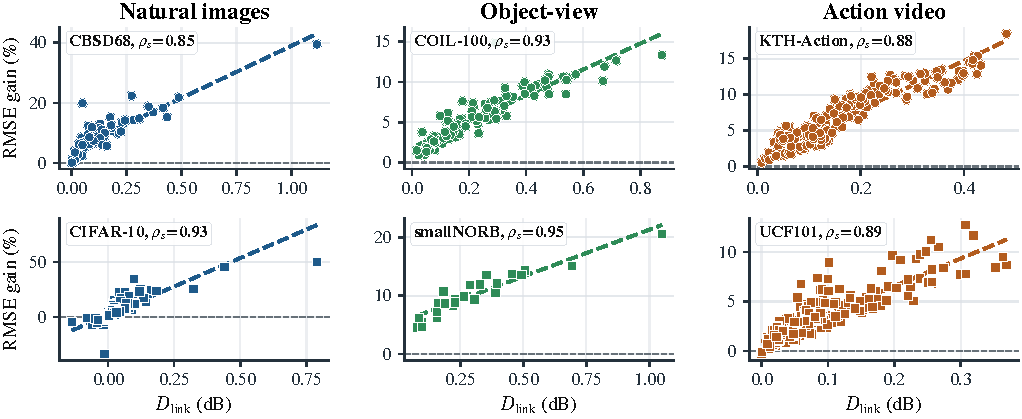
\includegraphics[width=\linewidth]{figures/nonhsi_dlink_scatter_3domain.pdf}
  \caption{Per-unit cross-domain diagnostic correlation. Each panel plots
  \(D_{\mathrm{link}}\) against NTD-PL RMSE gain over independently fitted
  tensor units. }
  \label{fig:nonhsi-link-scatter}
\end{figure}

These diagnostic results answer the third question. A single frozen-backbone Link Refresh score
is already predictive of where full NTD-PL will help, across both CAVE completion and non-HSI
tensor units. This supports the scoped claim of the paper: NTD-PL is useful when matched-rank
Tucker leaves residual structure that is coherent with a shared scalar response, and low diagnostic
yield correctly signals cases where the polynomial link should provide little benefit.

\FloatBarrier
